
\chapter{Version Control}

A version control system gives you automated help at keeping a change history for a file or group files.
It allows you to recover an stage in that directory, and it makes getting reports on the different between versions easy.

\section{How VC Helps with Basic Operations}

Historically, you had to know \keyword{three or four} different shell commands to do the basic operations of version control (registration, check in, check out, and revert).
This procedure was complicated and annoying, or at best a distraction from the flow of working on your code and changes.

VC's interface is much simpler.
The simplicity comes from noticing that whatever state your version-controlled file is in, there is normally just \keyword{one} logical thing to do next. 
Thus, VC mode has just one basic command: \verb|C-x v v| (for \verb|vc-next-action|), which you can think of as ``do the next logical thing to this file''.

\begin{figure}[H]
  \centering
  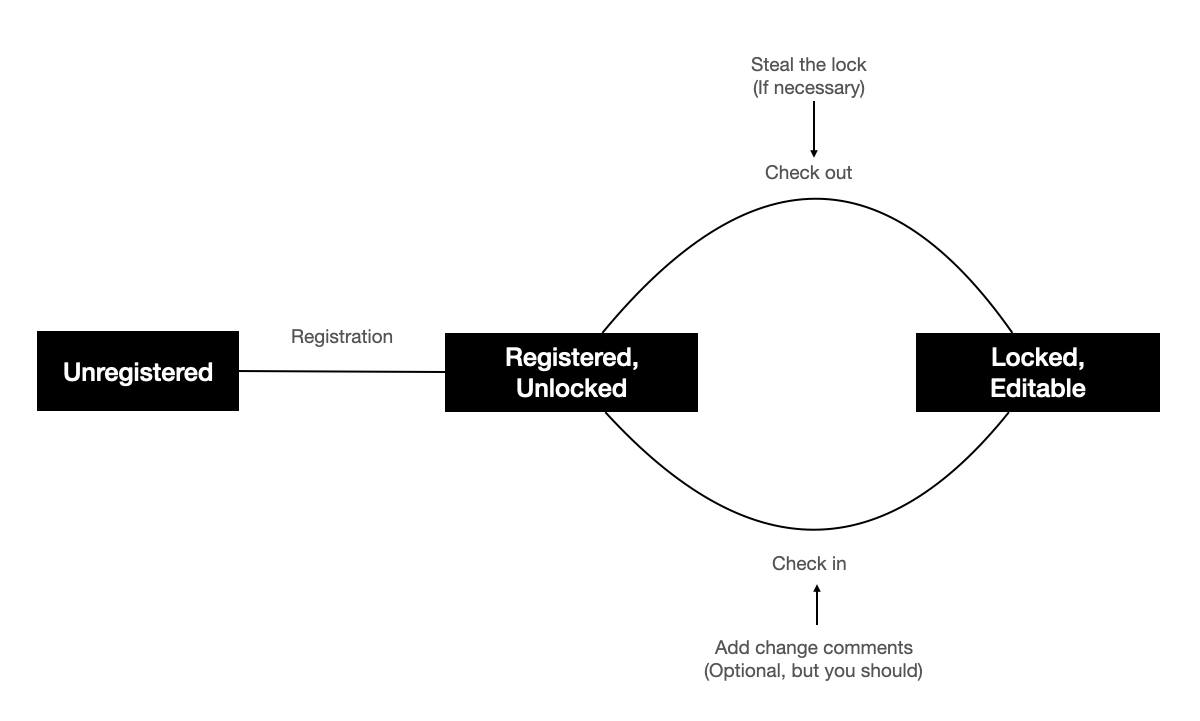
\includegraphics[width=0.9\textwidth]{vc.png}
  \caption{VC status}
\end{figure}

\section{Editing Comment Buffers}


In VC mode, three operations typically pop up a buffer to accept comment or notification text:
\begin{itemize}
\item check in
\item lock stealing
\item file registration
\end{itemize}
In each case, the operation is on hold until you type \verb|C-c C-c| to commit the comment buffer.


The comment buffer is a plain-text buffer.
However, each time you commit a comment buffer, the contents are saved to a new slot in a ring of comment buffers.
You can cycle backwards in the ring with \verb|M-p| and forward with \verb|M-n| , or you can search for text backwards in the ring with \verb|M-r| and forward with \verb|M-s| .
By design, these are the same keys you can use to navigate an Emacs minibuffer command history.

\section{VC Command Summary}

\begin{description}
\item[C-x v v] Go to the next logical version control state.
\item[C-x v d] Show all files beneath a directory.
\item[C-x v =] Display diffs between file revisions.
\item[C-x v u] Revert working copies of the selected fileset to their repository contents.
\item[C-x v ~] Visit revision REV of the current file in another window.
\item[C-x v l] Display a file's change comments and history.
\item[C-x v i] Register a file for version control.
\end{description}